
%------------------------------------------------------------%
\begin{frame}

\frametitle{Introduction to the Normal Distribution}
\begin{itemize}
\item
Recall the experiment whereby a die was rolled 100 times, and the sum of the 100 values was recorded.
\item
This experiment was repeated a very large number of times (e.g. 100,000 times ) in a simulation study.
\item
A histogram was drawn to depict the distribution of outcomes of this experiment.
\item Recall that we agreed that ``bell-shaped" was a good description of the histogram.

\end{itemize}
\end{frame}


\frame{
\frametitle{Normal Distribution}

\begin{center}
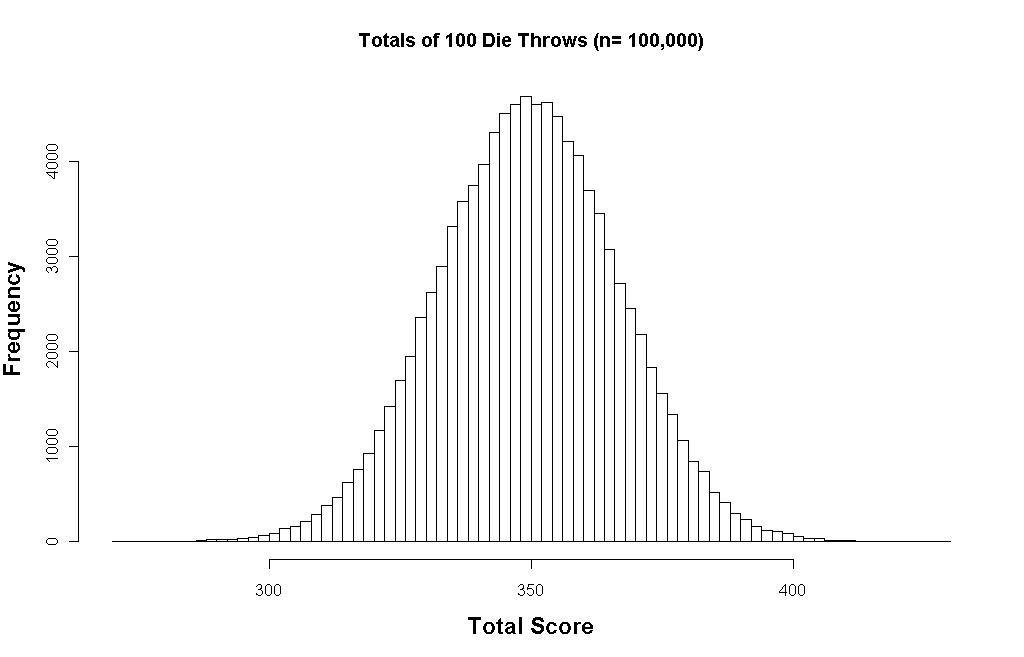
\includegraphics[scale=0.30]{3aDieHist3}
\end{center}

}
%----------------------------------------------------------------------%

\frame{
\frametitle{Normal Distribution}
\begin{itemize}
\item The normal distribution is perhaps the most widely used distribution for a random variable.
\item Normal distributions have the same general shape: the bell curve.
\item The distributions are \textbf{symmetric} with values concentrated more in the middle than in the tails.
%\item Examples of normal distributions are shown below. Notice that they differ in how spread out they are. The area under each curve is the same.
\item \alert{Important} The height of a normal distribution can be defined mathematically in terms of two fundamental parameters: the normal mean ($\mu$) and the normal
    standard deviation ($\sigma$).
\item A normally distributed random variable X is denoted $ X \sim \mbox{N} (\mu, \sigma^2)$ (note that we use the variance term here)
    \item The mean ($\mu$) and standard deviation ($\sigma$) are vital for calculating probabilities.
\end{itemize}
}
%------------------------------------------------------------------------%
\frame{
\frametitle{The Normal Distribution}
The \textbf{\emph{probability density function}} of the normal distribution is given as
\[ f(x) = \frac{1}{\sqrt{2\pi\sigma^2}} e^{ -\frac{(x-\mu)^2}{2\sigma^2} } \]

Integrating this formula would allow us to compute probabilities.
However, it is not required to use this formula.
}
%------------------------------------------------------------------%
\frame{
\frametitle{Normal Distribution}

\begin{center}
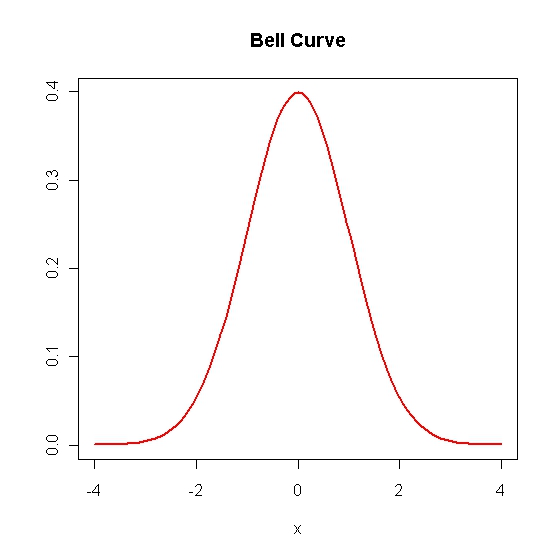
\includegraphics[scale=0.30]{5ABellCurve}
\end{center}

}
%%%%%%%%%%%%%%%%%%%%%%%%%%%%%%%%%%%%%%%%%%%%%%%%%%%%%%%%%%%%%%%%%%%%%%%%%%%%%%%%%%%%%%%%%%%%%%%%%%%%%%%%%%5


%------------------------------------------------------------------%
\frame{
\frametitle{Complement and Symmetry Rules}

Any normal distribution problem can be solved with some combination of the following rules.
\begin{itemize} \item \textbf{Complement rule} \item Common to all continuous random variables
\[P(Z \geq k) = 1 - P(Z \leq k) \]
Similarly
\[P(X \geq k) = 1 - P(X \leq k) \]
\end{itemize}

\[P(Z \leq 1.28) = 1 - P(Z \geq 1.28)  = 1-0.1003 = 0.8997\]
}

%------------------------------------------------------------------%
\frame{
\frametitle{Complement and Symmetry Rules}
\begin{itemize}
\item \textbf{Symmetry rule}
\item
This rule is based on the property of symmetry mentioned previously.
\item
Only the probabilities corresponding to values between 0 and 4 are tabulated in Murdoch Barnes.
\item
If we have a negative value of k, we can use the symmetry rule.
\end{itemize}
\[P(Z \leq -k) = P(Z \geq k) \]
by extension, we can say
\[P(Z \geq -k) = P(Z \leq k) \]
}
%------------------------------------------------------------------%
\frame{
\frametitle{Z Scores: Example 1 }
Find $P(Z \geq -1.28)$\\
\textbf{Solution}\\
\begin{itemize}
\item Using the symmetry rule
\[P(Z \geq -1.28) = P(Z \leq 1.28) \]
\item Using the complement rule
\[P(Z \geq -1.28) = 1 - P(Z \geq 1.28) \]
\[P(Z \geq -1.28) = 1 - 0.1003 = 0.8997 \]
\end{itemize}
}
%------------------------------------------------------------------%
\frame{
\frametitle{Z Scores: Example 2 }
Find the probability of a ``z" random variable being between -1.8 and 1.96?
i.e. Compute $P(-1.8 \leq Z \leq 1.96)$\\
Solution
\begin{itemize}
\item Consider the complement event of being in this interval: a combination of being too low or too high.
\item
The probability of being too low for this interval is $P(Z \leq -1.80) = 0.0359$ (check)
\item
The probability of being too high for this interval is $P(Z \geq 1.96) = 0.0250$ (check)
\item
Therefore the probability of being \textbf{outside} the interval is 0.0359 + 0.0250 = 0.0609.
\item
Therefore the probability of being \textbf{inside} the interval is 1- 0.0609 = 0.9391
$P(-1.8 \leq Z \leq 1.96) = 0.9391$
\end{itemize}
}

